\documentclass{standalone}
\usepackage{tikz}
\usetikzlibrary{patterns, positioning}

\begin{document}
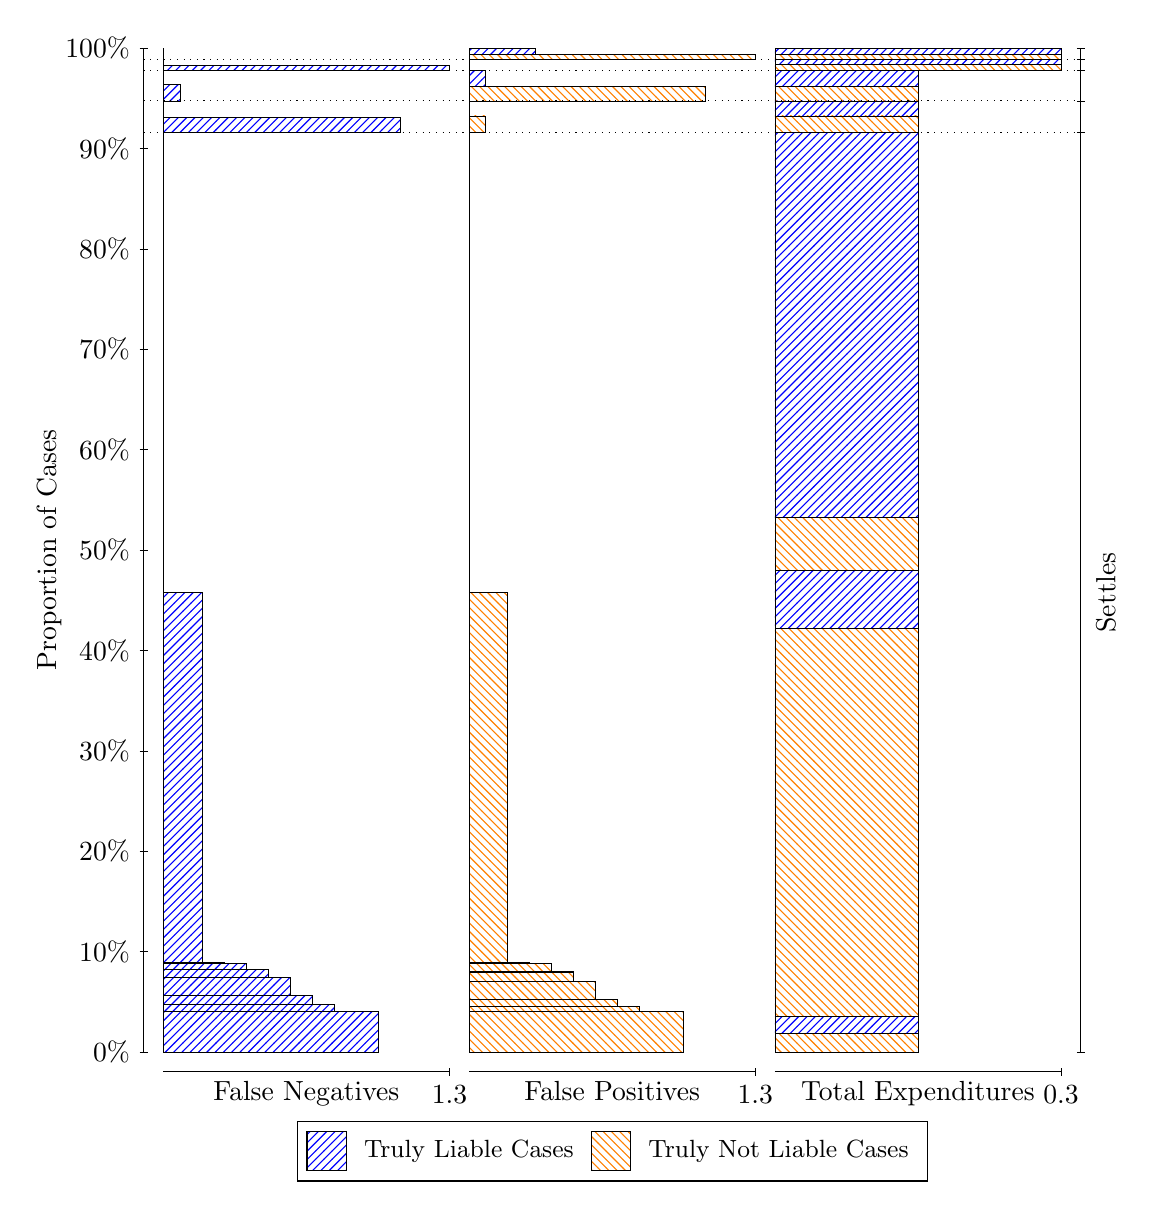
\begin{tikzpicture}
\draw[black, very thin] (1.5,1.75) -- (1.5,14.5);
\node[rotate=90, anchor=center] at (0.3, 8.125) {Proportion of Cases};
\draw[black, very thin] (1.45,1.75) -- (1.55,1.75);
\node[anchor=east] at (1.45, 1.75) {0\%};
\draw[black, very thin] (1.45,3.025) -- (1.55,3.025);
\node[anchor=east] at (1.45, 3.025) {10\%};
\draw[black, very thin] (1.45,4.3) -- (1.55,4.3);
\node[anchor=east] at (1.45, 4.3) {20\%};
\draw[black, very thin] (1.45,5.575) -- (1.55,5.575);
\node[anchor=east] at (1.45, 5.575) {30\%};
\draw[black, very thin] (1.45,6.85) -- (1.55,6.85);
\node[anchor=east] at (1.45, 6.85) {40\%};
\draw[black, very thin] (1.45,8.125) -- (1.55,8.125);
\node[anchor=east] at (1.45, 8.125) {50\%};
\draw[black, very thin] (1.45,9.4) -- (1.55,9.4);
\node[anchor=east] at (1.45, 9.4) {60\%};
\draw[black, very thin] (1.45,10.675) -- (1.55,10.675);
\node[anchor=east] at (1.45, 10.675) {70\%};
\draw[black, very thin] (1.45,11.95) -- (1.55,11.95);
\node[anchor=east] at (1.45, 11.95) {80\%};
\draw[black, very thin] (1.45,13.225) -- (1.55,13.225);
\node[anchor=east] at (1.45, 13.225) {90\%};
\draw[black, very thin] (1.45,14.5) -- (1.55,14.5);
\node[anchor=east] at (1.45, 14.5) {100\%};

\draw[black, very thin] (13.4,1.75) -- (13.4,14.5);
\draw[black, very thin] (13.35,1.75) -- (13.45,1.75);
\node[anchor=west] at (13.35, 1.75) {};
\draw[black, very thin] (13.35,13.425) -- (13.45,13.425);
\node[anchor=west] at (13.35, 13.425) {};
\draw[black, very thin] (13.35,13.83) -- (13.45,13.83);
\node[anchor=west] at (13.35, 13.83) {};
\draw[black, very thin] (13.35,14.22) -- (13.45,14.22);
\node[anchor=west] at (13.35, 14.22) {};
\draw[black, very thin] (13.35,14.359) -- (13.45,14.359);
\node[anchor=west] at (13.35, 14.359) {};
\draw[black, very thin] (13.35,14.5) -- (13.45,14.5);
\node[anchor=west] at (13.35, 14.5) {};

\draw[black, very thin, pattern color=blue, pattern=north east lines] (1.75,1.75) rectangle (4.475,2.2612);
\draw[black, very thin, pattern color=blue, pattern=north east lines] (1.75,2.2612) rectangle (4.1955,2.2704);
\draw[black, very thin, pattern color=blue, pattern=north east lines] (1.75,2.2704) rectangle (3.916,2.3558);
\draw[black, very thin, pattern color=blue, pattern=north east lines] (1.75,2.3558) rectangle (3.6365,2.4695);
\draw[black, very thin, pattern color=blue, pattern=north east lines] (1.75,2.4695) rectangle (3.3571,2.6982);
\draw[black, very thin, pattern color=blue, pattern=north east lines] (1.75,2.6982) rectangle (3.0776,2.8006);
\draw[black, very thin, pattern color=blue, pattern=north east lines] (1.75,2.8006) rectangle (2.7981,2.8744);
\draw[black, very thin, pattern color=blue, pattern=north east lines] (1.75,2.8744) rectangle (2.5186,2.8898);
\draw[black, very thin, pattern color=blue, pattern=north east lines] (1.75,2.8898) rectangle (2.2391,7.5876);
\draw[black, very thin, pattern color=orange, pattern=north west lines] (1.75,7.5876) rectangle (1.75,13.425);
\draw[black, very thin, pattern color=blue, pattern=north east lines] (1.75,13.425) rectangle (4.7545,13.617);
\draw[black, very thin, pattern color=orange, pattern=north west lines] (1.75,13.617) rectangle (1.75,13.83);
\draw[black, very thin, pattern color=blue, pattern=north east lines] (1.75,13.83) rectangle (1.9596,14.035);
\draw[black, very thin, pattern color=orange, pattern=north west lines] (1.75,14.035) rectangle (1.75,14.22);
\draw[black, very thin, pattern color=blue, pattern=north east lines] (1.75,14.22) rectangle (5.3833,14.282);
\draw[black, very thin, pattern color=orange, pattern=north west lines] (1.75,14.282) rectangle (1.75,14.359);
\draw[black, very thin, pattern color=orange, pattern=north west lines] (1.75,14.359) rectangle (1.75,14.422);
\draw[black, very thin, pattern color=blue, pattern=north east lines] (1.75,14.422) rectangle (1.75,14.5);
\draw[black, very thin, pattern color=orange, pattern=north west lines] (5.6333,1.75) rectangle (8.3583,2.2612);
\draw[black, very thin, pattern color=orange, pattern=north west lines] (5.6333,2.2612) rectangle (8.0788,2.2685);
\draw[black, very thin, pattern color=orange, pattern=north west lines] (5.6333,2.2685) rectangle (7.7994,2.3271);
\draw[black, very thin, pattern color=orange, pattern=north west lines] (5.6333,2.3271) rectangle (7.5199,2.4202);
\draw[black, very thin, pattern color=orange, pattern=north west lines] (5.6333,2.4202) rectangle (7.2404,2.6489);
\draw[black, very thin, pattern color=orange, pattern=north west lines] (5.6333,2.6489) rectangle (6.9609,2.756);
\draw[black, very thin, pattern color=orange, pattern=north west lines] (5.6333,2.756) rectangle (6.9609,2.7699);
\draw[black, very thin, pattern color=orange, pattern=north west lines] (5.6333,2.7699) rectangle (6.6814,2.8704);
\draw[black, very thin, pattern color=orange, pattern=north west lines] (5.6333,2.8704) rectangle (6.4019,2.8897);
\draw[black, very thin, pattern color=orange, pattern=north west lines] (5.6333,2.8897) rectangle (6.1224,7.5876);
\draw[black, very thin, pattern color=blue, pattern=north east lines] (5.6333,7.5876) rectangle (5.6333,13.425);
\draw[black, very thin, pattern color=orange, pattern=north west lines] (5.6333,13.425) rectangle (5.8429,13.639);
\draw[black, very thin, pattern color=blue, pattern=north east lines] (5.6333,13.639) rectangle (5.6333,13.83);
\draw[black, very thin, pattern color=orange, pattern=north west lines] (5.6333,13.83) rectangle (8.6378,14.015);
\draw[black, very thin, pattern color=blue, pattern=north east lines] (5.6333,14.015) rectangle (5.8429,14.22);
\draw[black, very thin, pattern color=orange, pattern=north west lines] (5.6333,14.22) rectangle (5.6333,14.297);
\draw[black, very thin, pattern color=blue, pattern=north east lines] (5.6333,14.297) rectangle (5.6333,14.359);
\draw[black, very thin, pattern color=orange, pattern=north west lines] (5.6333,14.359) rectangle (9.2667,14.422);
\draw[black, very thin, pattern color=blue, pattern=north east lines] (5.6333,14.422) rectangle (6.4718,14.5);
\draw[black, very thin, pattern color=orange, pattern=north west lines] (9.5167,1.75) rectangle (11.333,1.9909);
\draw[black, very thin, pattern color=blue, pattern=north east lines] (9.5167,1.9909) rectangle (11.333,2.1992);
\draw[black, very thin, pattern color=orange, pattern=north west lines] (9.5167,2.1992) rectangle (11.333,7.1257);
\draw[black, very thin, pattern color=blue, pattern=north east lines] (9.5167,7.1257) rectangle (11.333,7.8655);
\draw[black, very thin, pattern color=orange, pattern=north west lines] (9.5167,7.8655) rectangle (11.333,8.5357);
\draw[black, very thin, pattern color=blue, pattern=north east lines] (9.5167,8.5357) rectangle (11.333,13.425);
\draw[black, very thin, pattern color=orange, pattern=north west lines] (9.5167,13.425) rectangle (11.333,13.639);
\draw[black, very thin, pattern color=blue, pattern=north east lines] (9.5167,13.639) rectangle (11.333,13.83);
\draw[black, very thin, pattern color=orange, pattern=north west lines] (9.5167,13.83) rectangle (11.333,14.015);
\draw[black, very thin, pattern color=blue, pattern=north east lines] (9.5167,14.015) rectangle (11.333,14.22);
\draw[black, very thin, pattern color=orange, pattern=north west lines] (9.5167,14.22) rectangle (13.15,14.297);
\draw[black, very thin, pattern color=blue, pattern=north east lines] (9.5167,14.297) rectangle (13.15,14.359);
\draw[black, very thin, pattern color=orange, pattern=north west lines] (9.5167,14.359) rectangle (13.15,14.422);
\draw[black, very thin, pattern color=blue, pattern=north east lines] (9.5167,14.422) rectangle (13.15,14.5);
\draw[black, dotted] (1.5,13.425) -- (13.4,13.425);
\draw[black, dotted] (1.5,13.83) -- (13.4,13.83);
\draw[black, dotted] (1.5,14.22) -- (13.4,14.22);
\draw[black, dotted] (1.5,14.359) -- (13.4,14.359);
\draw[black, very thin] (1.75,1.5) -- (5.3833,1.5);
\node[anchor=north] at (3.5667, 1.5) {False Negatives};
\draw[black, very thin] (5.3833,1.45) -- (5.3833,1.55);
\node[anchor=north] at (5.3833, 1.45) {1.3};

\draw[black, very thin] (5.6333,1.5) -- (9.2667,1.5);
\node[anchor=north] at (7.45, 1.5) {False Positives};
\draw[black, very thin] (9.2667,1.45) -- (9.2667,1.55);
\node[anchor=north] at (9.2667, 1.45) {1.3};

\draw[black, very thin] (9.5167,1.5) -- (13.15,1.5);
\node[anchor=north] at (11.333, 1.5) {Total Expenditures};
\draw[black, very thin] (13.15,1.45) -- (13.15,1.55);
\node[anchor=north] at (13.15, 1.45) {0.3};

\node[black, centered, rotate=90] at (13.72, 7.5876) {Settles};





\draw (7.449999999999999,1.5) node[draw=none] (baseCoordinate) {};
\begin{scope}[align=center]
        \matrix[scale=0.5, draw=black, below=0.5cm of baseCoordinate, nodes={draw}, column sep=0.1cm]{
            \node[rectangle, draw, minimum width=0.5cm, minimum height=0.5cm, pattern=north east lines, pattern color=blue] {}; &
            \node[draw=none, font=\small] (B) {Truly Liable Cases}; &
            \node[rectangle, draw, minimum width=0.5cm, minimum height=0.5cm, pattern=north west lines, pattern color=orange] {}; &
            \node[draw=none, font=\small] (B) {Truly Not Liable Cases}; \\
            };
\end{scope}

\end{tikzpicture}
\end{document}